% preamble and style file for M&R lecture slides
\documentclass[11.5pt,sans,english]{beamer}

\usetheme{EastLansing}
\usecolortheme{lily}

\usepackage[most]{tcolorbox}

\usepackage{verbatim}
%\usepackage{ulem}
%\usepackage{fontawesome}
%\usepackage{tikz}
%\usepackage{pifont}
%\usepackage{tabularx}
\usepackage{array,booktabs,xcolor,colortbl,multirow,rotating,amssymb}
%\usepackage{amsmath}
% \usepackage{vwcol}
% \usepackage[T1]{fontenc}

  
\newcommand\vect[1]{\underline{\mathbf{#1}}}
\newcommand\unitvect[1]{\hat{\boldsymbol{#1}}}
%\newcommand\hatdot[1] { \hat{ \dot{ \boldsymbol{#1} } } }

\newtcbox
{\keyc}{on line,arc=2pt, colback=yellow!30!white, colframe=yellow!30!black, before upper={\rule[-3pt]{0pt}{10pt} },boxrule=1pt,boxsep=0pt,left=6pt,right=6pt,top=2pt,bottom=2pt,}

\newtcbox
{\keyb}{on line,arc=1pt, colback=blue!30!white, colframe=blue!30!black, before upper={\rule[-3pt]{0pt}{10pt} },boxrule=1pt,boxsep=0pt,left=6pt,right=6pt,top=2pt,bottom=2pt,}

\newtcbox
{\keyl}{on line,arc=1pt, colback=pink!30!white, colframe=blue!30!black, before upper={\rule[-3pt]{0pt}{10pt} },boxrule=1pt,boxsep=0pt,left=6pt,right=6pt,top=2pt,bottom=2pt,}

\newtcbox
{\keyw}{on line,arc=1pt, colback=red!30!white, colframe=blue!30!black, before upper={\rule[-3pt]{0pt}{10pt} },boxrule=1pt,boxsep=0pt,left=6pt,right=6pt,top=2pt,bottom=2pt,}

\newtcbox
{\keya}{on line,arc=1pt, colback=purple!30!white, colframe=blue!30!black, before upper={\rule[-3pt]{0pt}{10pt} },boxrule=1pt,boxsep=0pt,left=6pt,right=6pt,top=2pt,bottom=2pt,}

\newtcbox[auto counter,number within=section]
{keyf}
{
enhanced,
on line,
  boxsep=0pt,
  left=6pt,right=6pt,top=2pt,bottom=2pt,
  arc=5pt,
  boxrule=1pt,
  rightrule=38pt,
colback=green!10!white, 
colframe=green!50!black, 
title=\thetcbcounter,
detach title,
overlay unbroken and first ={
    \node[%rotate=90,
          %minimum width=1cm,
          anchor=south,
          font=\sffamily\bfseries\tiny,
          %yshift=-10pt,
          yshift=-5pt,
          xshift=-20pt,
          white]
    at (frame.east) {\thetcbcounter};
  }
}


\usepackage{xcolor}

%\usepackage{hyperref}
%\hypersetup{
%  pdfauthor={Lily Asquith},
%  urlcolor=blue,
%  colorlinks=true,
%  linkcolor=blue,
%  bookmarks=true
%}

%---------------------------------------------%
%              LILY'S COLOURS           %
%---------------------------------------------%
\definecolor{Wash}{RGB}{204,204,204}
%\definecolor{Pinky}{RGB}{254,200,254}%violet
\definecolor{Pinky}{RGB}{219,	240,	253}%violet
\definecolor{Bluey}{RGB}{0,190,255}%deep sky blue
\definecolor{DarkGrey}{RGB}{28,66,137}%dar grey
\definecolor{SussexWhite}{RGB}{253,255,254}%dar grey
\definecolor{LightGray}{RGB}{184,184,255}
\definecolor{YesGreen}{RGB}{0,128,0}
\definecolor{NoRed}{RGB}{250,0,0}



\definecolor{myred}{RGB}{255,153,153}
\definecolor{myorange}{RGB}{255,204,153}
\definecolor{myyellow}{RGB}{255,255,153}
\definecolor{mygreen}{RGB}{153,255,153}
\definecolor{mycyan}{RGB}{153,255,255}
\definecolor{myblue}{RGB}{153,204,255}
\definecolor{myviolet}{RGB}{153,153,255}
\definecolor{mypurple}{RGB}{204,153,255}
\definecolor{mypink}{RGB}{255,204,255}
\definecolor{mycoral}{RGB}{255,153,204}

%-----------------------------------------------------%
%              LILY'S COLUMN TYPES          %
%-----------------------------------------------------%
\newcolumntype{a}{>{\raggedright\arraybackslash}l}	
\newcolumntype{q}{>{\raggedright\arraybackslash}m{8cm}} 

%--------------------------------------------%
%              LILY'S SYMBOLS          %
%--------------------------------------------%
\newcommand{\dfinger}{\large{\textcolor{black}{\ding{43}}}\scriptsize}
\newcommand{\dstar}{\large{\textcolor{black}{\ding{76}}}\scriptsize}
\newcommand{\dwrite}{\large{\textcolor{black}{\ding{45}}}\scriptsize}
\newcommand{\ddiamond}{\small{\textcolor{DarkGrey}{\ding{117}}}\scriptsize}
\newcommand{\ddiamondwhite}{\small{\textcolor{SussexWhite}{\ding{117}}}\scriptsize}
\newcommand{\experiment}{\small{\textcolor{magenta}{\faCogs }}\scriptsize}
\newcommand{\watchit}{\textcolor{blue}{ \faYoutube}}


\makeatletter
\newcommand\notsotiny{\@setfontsize\notsotiny{6.5}{7.5}}
\makeatother


% 
\title[ Mechanics \& Relativity]{Mechanics \& Relativity}
%\subtitle{\textbf{Topic 1: Kinematics }}
\author[Dr Lily Asquith (Lily)]{ Dr Lily Asquith (Lily)}
\date[Week 4]{Week 4}
\logo{

\includegraphics[width=1.5cm]{../../utils/uslogo.jpg}
}


\begin{document}


\begin{frame}
\titlepage
\end{frame} 



 %-----------------------------------------------------------%
 % 1 Relative Motion                                              %
 %-----------------------------------------------------------%
\section{M\&R 4: Forces 1}
\begin{frame}
\frametitle{Forces 1} 
\normalsize

This week's topics:\\[3ex]

\begin{itemize}
\item[4.1] Relative Motion\\[3ex]
\item[4.2] Newton's Laws\\[3ex]
\item[4.3] Problem Solving\\[3ex]
\end{itemize}
\end{frame} 
 

\begin{frame}{Frames of Reference}
\small
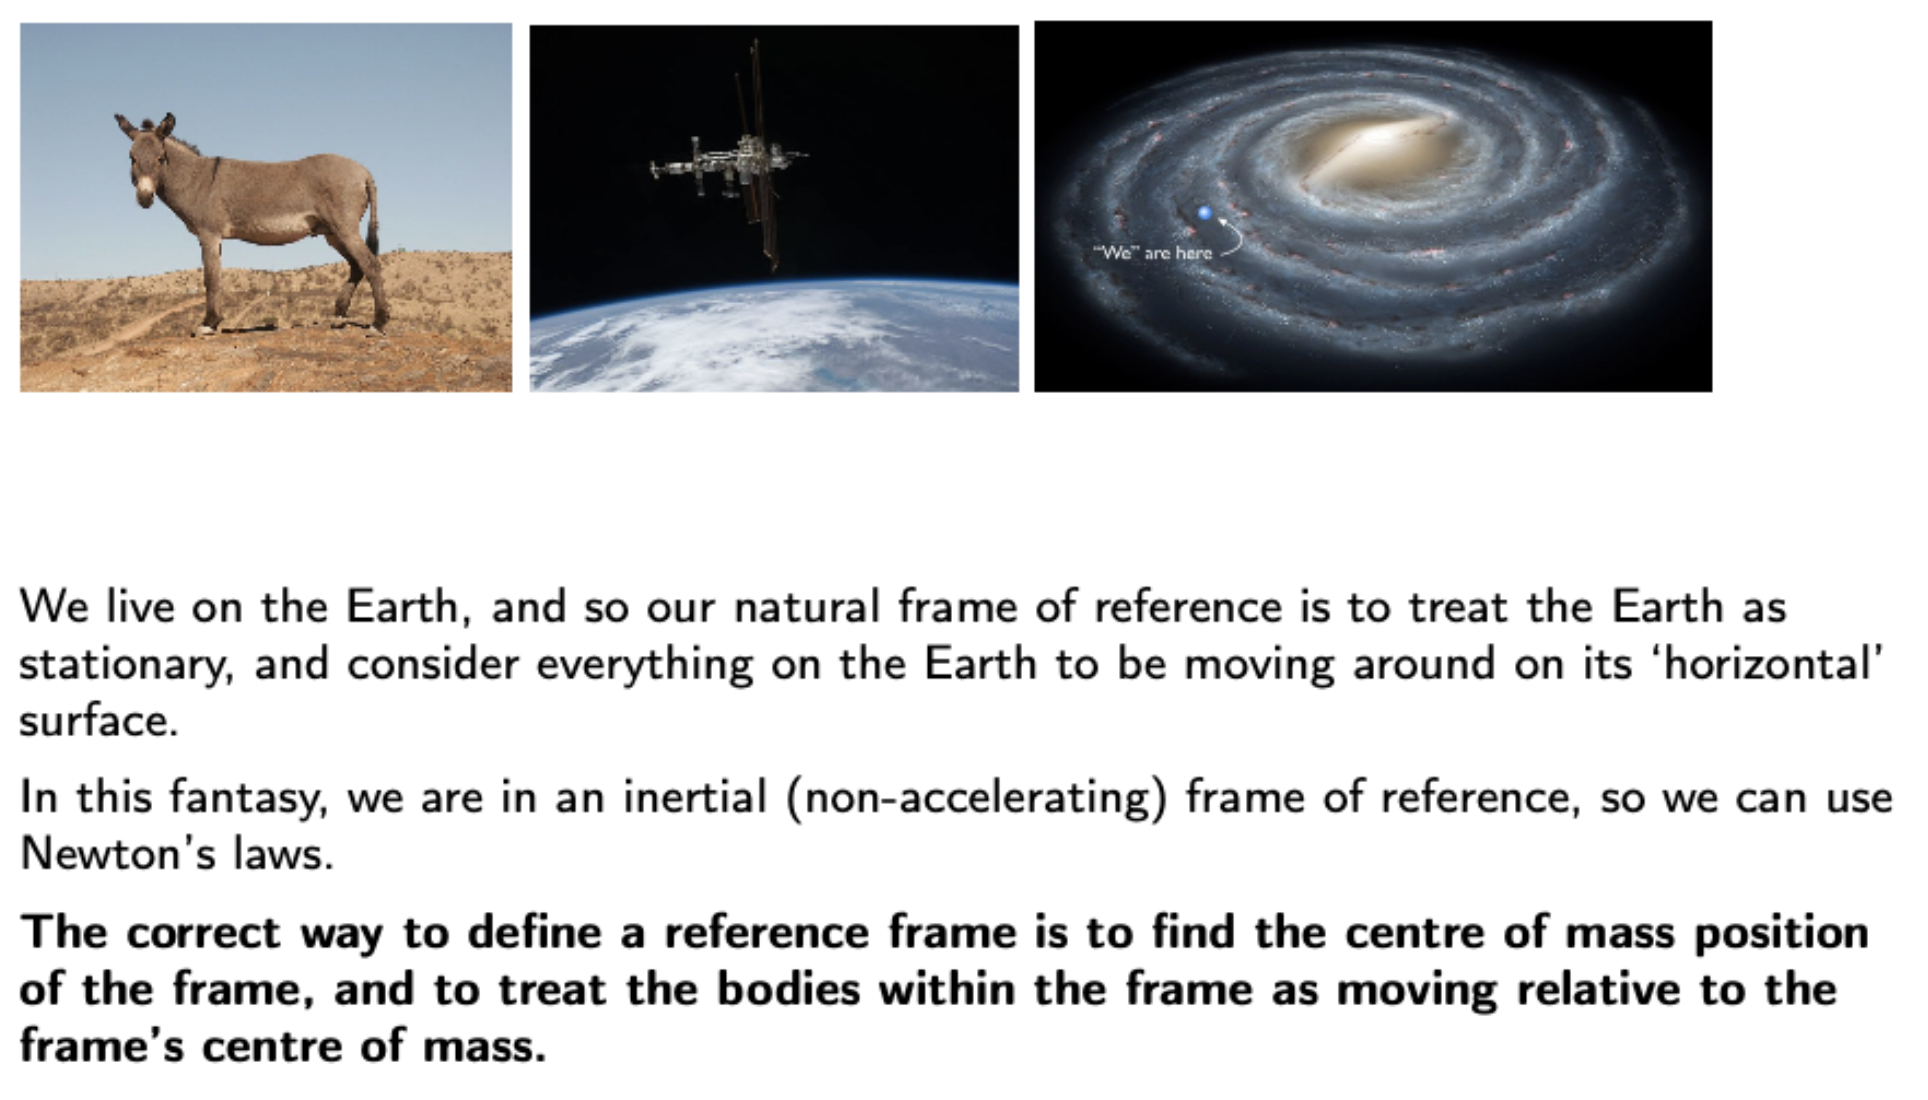
\includegraphics[scale=0.34]{frames-intro}
\vspace{10cm}
\end{frame}



 \subsection{Relative Motion}
%\begin{frame}{Relative Motion}
%\small
%The same laws of physics apply in any \textit{reference frame} which is moving at constant velocity with respect to Earth.\\[1ex]
%\vspace{10cm}
%\end{frame}

\begin{frame}{Relative Motion}
\small
To do calculations across different inertial reference frames, we need to consider their relative motion.\\
\vspace{10cm}
\end{frame}

\begin{frame}{Example: plane-air-ground}
\small
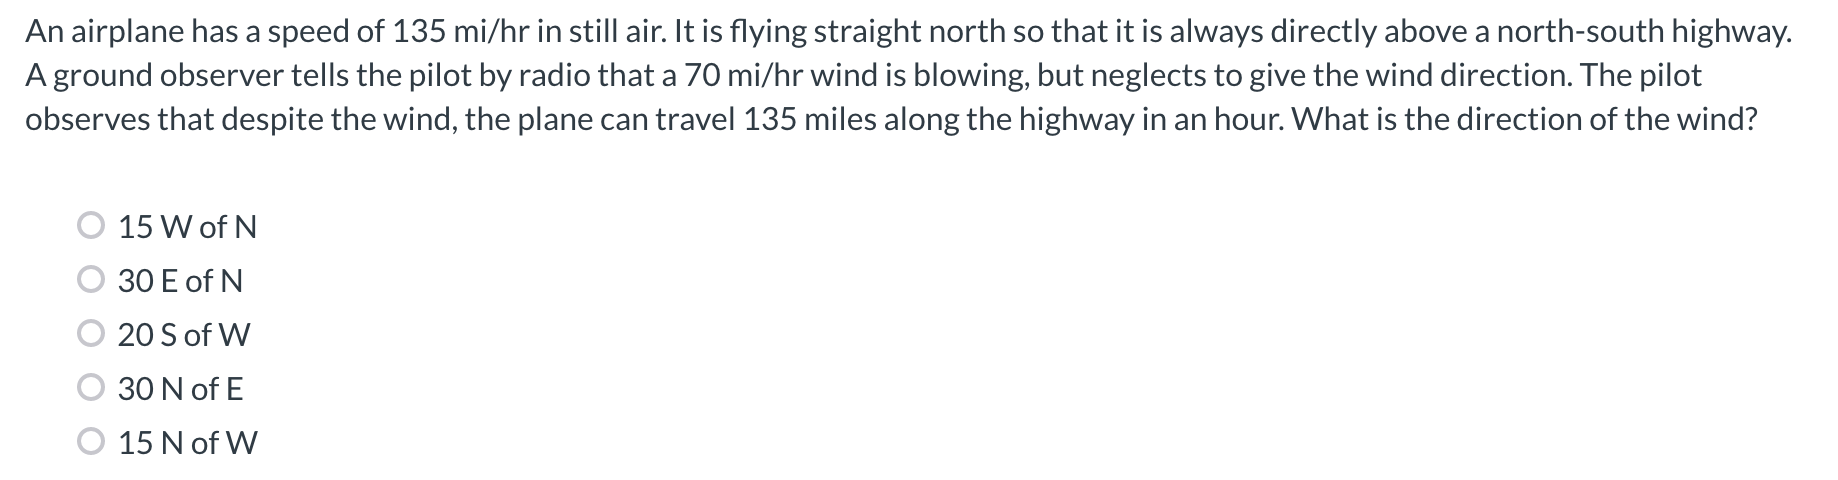
\includegraphics[scale=0.35]{plane-problem}

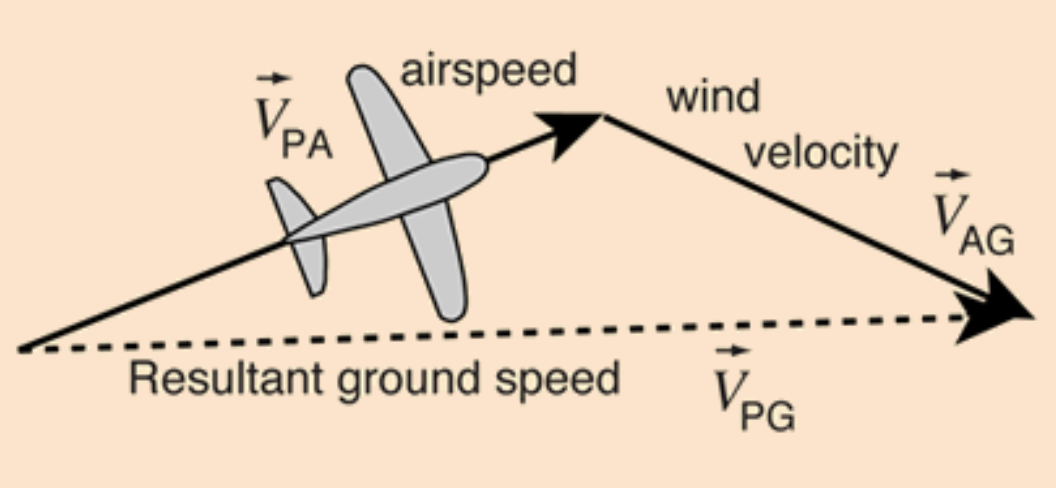
\includegraphics[scale=0.3]{plane}

\vspace{5cm}
\end{frame}

 
\begin{frame}{Example: ball-person-ground}
\scriptsize
A rugby player runs with the ball directly toward his opponent's goal, along the positive direction of an x axis. He can legally pass the ball to a teammate as long as the ball's velocity relative to the field does not have a positive x component. Suppose the player runs at speed 4.0 m/s relative to the field while he passes the ball with velocity $\vect{v}_{BP}$ relative to himself. If $\vect{v}_{BP}$ has magnitude 6.0 m/s, what is the smallest angle it can have for the pass to be legal?
\vspace{5cm}
\end{frame}


 \begin{frame}{Example: boat-river-ground}
\notsotiny
A 200-m-wide river has a uniform flow speed of 1.1 m/s through a jungle and toward the east. An explorer wishes to leave a small clearing on the south bank and cross the river in a powerboat that moves at a constant speed of 4.0 m/s with respect to the water. There is a clearing on the north bank 82 m upstream from a point directly opposite the clearing on the south bank. (a) In what direction must the boat be pointed in order to travel in a straight line and land in the clearing on the north bank? (b) How long will the boat take to cross the river and land in the clearing?
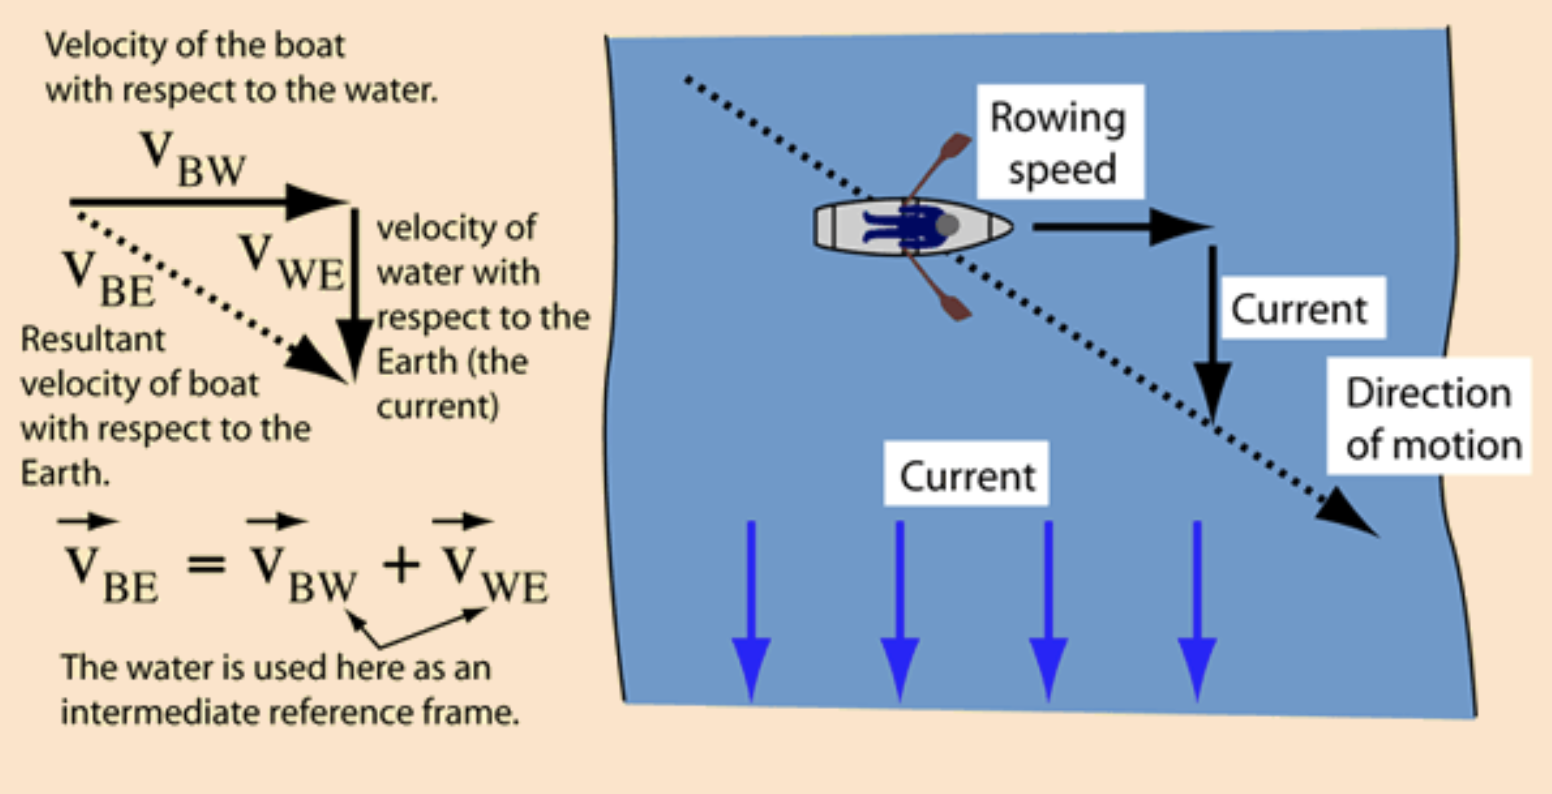
\includegraphics[scale=0.3]{boat}%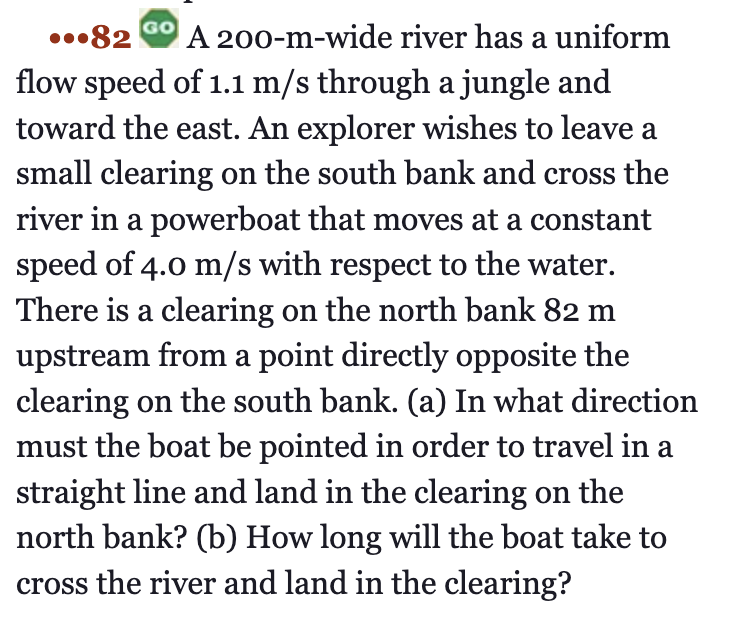
\includegraphics[scale=0.5]{river}
\vspace{5cm}
\end{frame}


 \begin{frame}{Example: boat-river-ground}
\notsotiny
A 200-m-wide river has a uniform flow speed of 1.1 m/s through a jungle and toward the east. An explorer wishes to leave a small clearing on the south bank and cross the river in a powerboat that moves at a constant speed of 4.0 m/s with respect to the water. There is a clearing on the north bank 82 m upstream from a point directly opposite the clearing on the south bank. (a) In what direction must the boat be pointed in order to travel in a straight line and land in the clearing on the north bank? (b) How long will the boat take to cross the river and land in the clearing?

\vspace{8cm}
\end{frame}

%%%%%%%%
 \subsection{Newton's Laws}
 
 
 \begin{frame}{Most hated problem from AP 4.2}
\small


\end{frame}


\begin{frame}{Newton's First and Second Laws}
\small
N1: If there is no \textbf{net external force} acting on me, I will remain at my current velocity forever.\\[2ex]
N2: $\vect{F} = m \vect{a}$ \\[1ex]
\vspace{10cm}

\end{frame}

\begin{frame}{N1: Two forces acting on a particle}
\small
While two forces act on it, a particle is to move at the constant velocity 
$\vect{v} = (3ms^{-1})\unitvect{i} - (4ms^{-1})\unitvect{j}$.\\
One of the forces is $\vect{F} = (2N)\unitvect{i} - (6N)\unitvect{j}$. What is the other force?
\vspace{10cm}
\end{frame}


\begin{frame}{N2: Blocks \& Pulleys}
\scriptsize
A block S with mass $M_s = 3.3$ kg is free to move along a horizontal frictionless surface and is connected, by a cord that wraps over a frictionless pulley, to a second block H with mass $M_h = 2.1$ kg. The cord and pulley have negligible masses. \\
Find (a) the acceleration of block S, (b) the acceleration of block H, and (c) the tension in the cord.

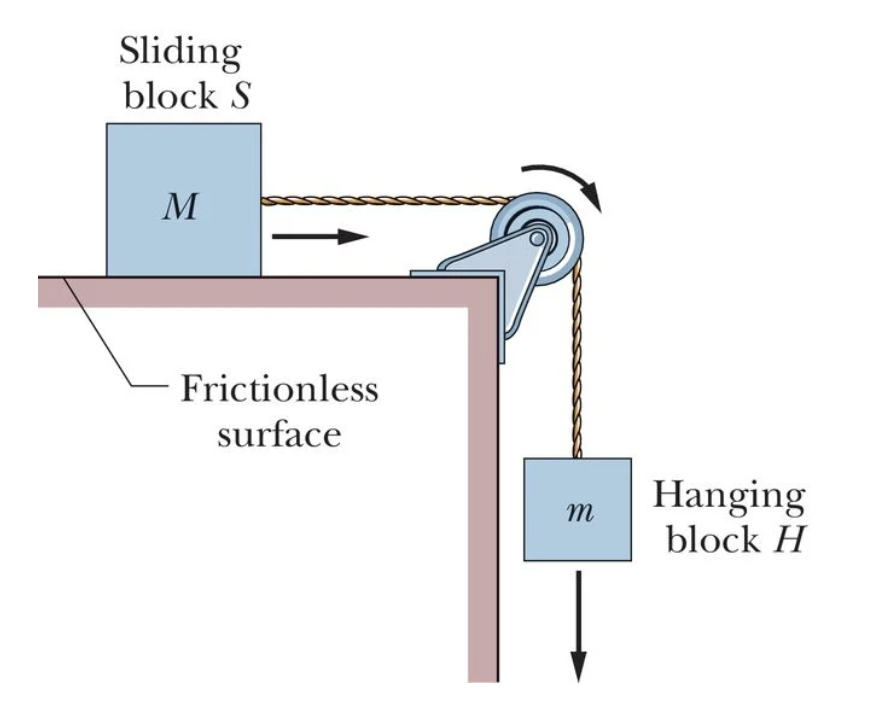
\includegraphics[scale=0.3]{block-pulley-1}
\vspace{8cm}
\end{frame}


\begin{frame}{N2: Boxes \& Ramps}
\scriptsize
A cord pulls a box of biscuits up along a frictionless plane inclined at angle $\theta = 30.0^{\circ}$. The box has mass m = 5.00 kg, and the force from the cord has magnitude T = 25.0 N. What is the box's acceleration along the inclined plane?
\vspace{8cm}
\end{frame}


\begin{frame}{N2: Inside a lift}
\scriptsize
A passenger of mass m = 72.2 kg stands on a weighing scale in a lift. We are concerned with the scale readings when the cab is stationary and when it is moving up or down.  Find a general solution for the scale reading, whatever the vertical motion of the cab.
\vspace{8cm}
\end{frame}


\begin{frame}{N2: Block pushing Block}
\scriptsize
A constant horizontal force of magnitude 20 N is applied to block A of mass mA = 4.0 kg, which pushes against block B of mass mB = 6.0 kg. The blocks slide over a frictionless surface, along an x axis. (a) What is the acceleration of the blocks? (b) What is the force on block B from block A?
\vspace{8cm}
\end{frame}





%\begin{frame}{Another Problem, with free body diagrams}
%\small
%A lift with total (lift + occupants) mass $M_{L} = 500 kg$ is moving upwards at constant velocity. What is the tension in the cable?\\[3ex]
%
%\vspace{10cm}
%\end{frame}
%
%
%\begin{frame}{Another Problem, with free body diagrams}
%\small
%A lift with total (lift + occupants) mass $M_{L} = 500 kg$ is moving upwards at constant velocity. What is the tension in the cable?\\[1ex]
%The same lift starts to accelerate downwards at 4 ms$^{-2}$. What is the tension in the cable?\\[3ex]
%
%\vspace{10cm}
%\end{frame}
%
%
%\begin{frame}{Another Problem, with free body diagrams}
%\small
%A lift with total (lift + occupants) mass $M_{L} = 500 kg$ is moving upwards at constant velocity. What is the tension in the cable?\\[1ex]
%The same lift starts to accelerate downwards at 4 ms$^{-2}$. What is the tension in the cable?\\[1ex]
%The lift is reset to some unknown motion. An occupant of the lift drops a coin, which accelerates downward at 4 ms$^{-2}$. What is the tension in the cable?\\[1ex]
%
%
%\vspace{10cm}
%\end{frame}


\begin{frame}{Newton's Third Law}
\small
N3: $\vect{F}_{AB} = - \vect{F}_{BA} $ \\[1ex]
\vspace{10cm}

\end{frame}

\begin{frame}{N3: Equal and opposite forces}
\small
The earth has mass $M_{E} = 6 \times 10^{24}$ kg. A large, sleepy dog has mass $M_{D} = 6\times10^1$ kg.\\[1ex]

What is the acceleration of the Earth due to the Dog?\\[1ex]

\vspace{10cm}

\end{frame}







\subsection{Problems}

 \begin{frame}{Most hated problem from AP 4.3}
\small


\end{frame}

\begin{frame}{Hanging disks in series}
\scriptsize
Four disks are suspended by cords. The longer, top cord loops over a frictionless pulley and pulls with a force of magnitude 98 N on the wall to which it is attached. The tensions in the three shorter cords are T1 = 58.8 N, T2 = 49.0 N, and T3 = 9.8 N. What are the masses of each of the disks?

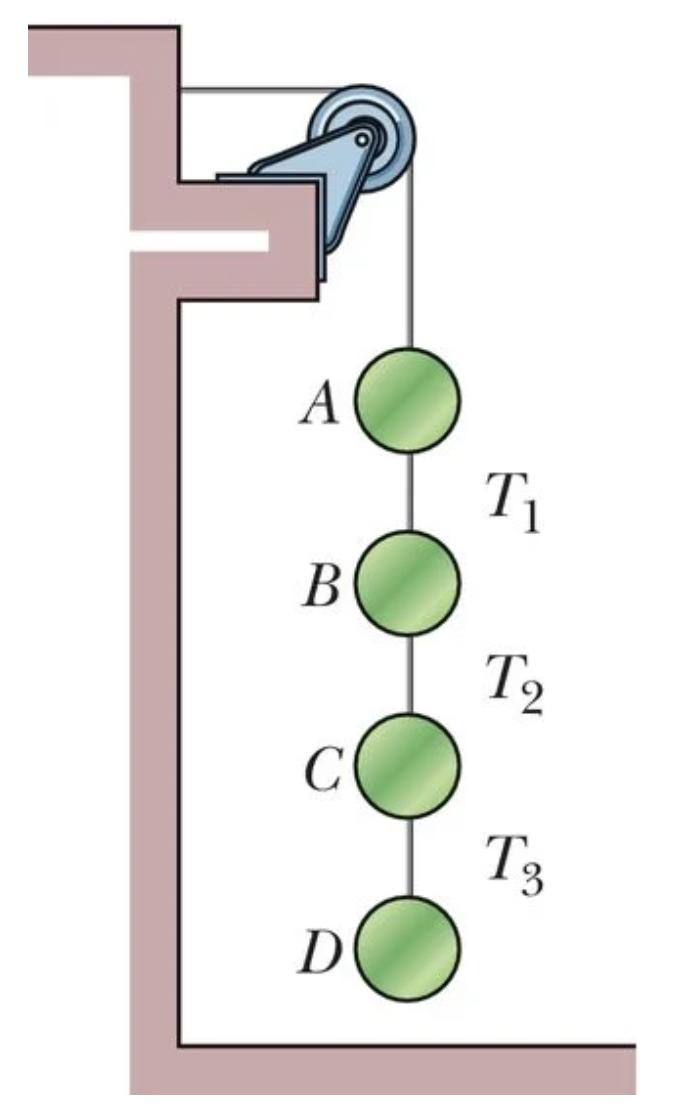
\includegraphics[scale=0.3]{disks}
\end{frame}

\begin{frame}{Crate problem}
\scriptsize
A crate of mass m = 100 kg is pushed at constant speed up a frictionless ramp ($\theta = 30.0^{\circ}$) by a horizontal force $\vect{F}$ . What are the magnitudes of (a) $\vect{F}$ and (b) the force on the crate from the ramp?

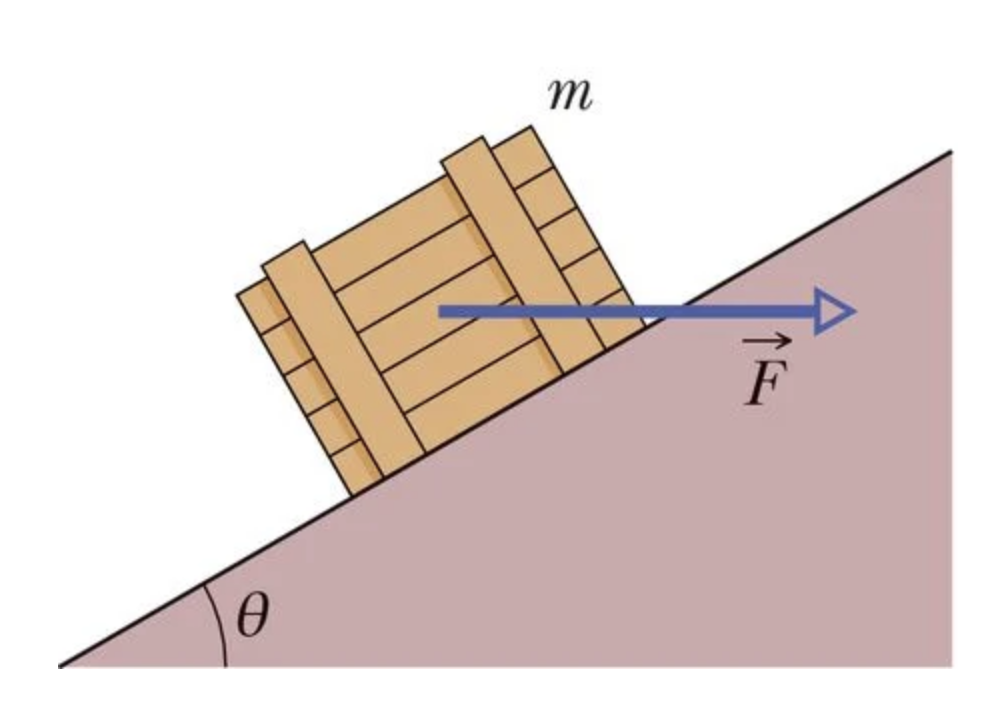
\includegraphics[scale=0.3]{crate2}
\vspace{4cm}
\end{frame}


\begin{frame}{Pulley Problem that messes with Lily's brain}
\scriptsize
A man sitting in a bosun's chair that dangles from a massless rope, which runs over a massless, frictionless pulley and back down to the man?s hand. The combined mass of man and chair is 95.0 kg. With what force magnitude must the man pull on the rope if he is to rise (a) with a constant velocity and (b) with an upward acceleration of 1.30 ms$^{-2}$? 

% If the rope on the right extends to the ground and is pulled by a co-worker, with what force magnitude must the co-worker pull for the man to rise (c) with a constant velocity and (d) with an upward acceleration of 1.30 m/s2? What is the magnitude of the force on the ceiling from the pulley system in (e) part a, (f) part b, (g) part c, and (h) part d?


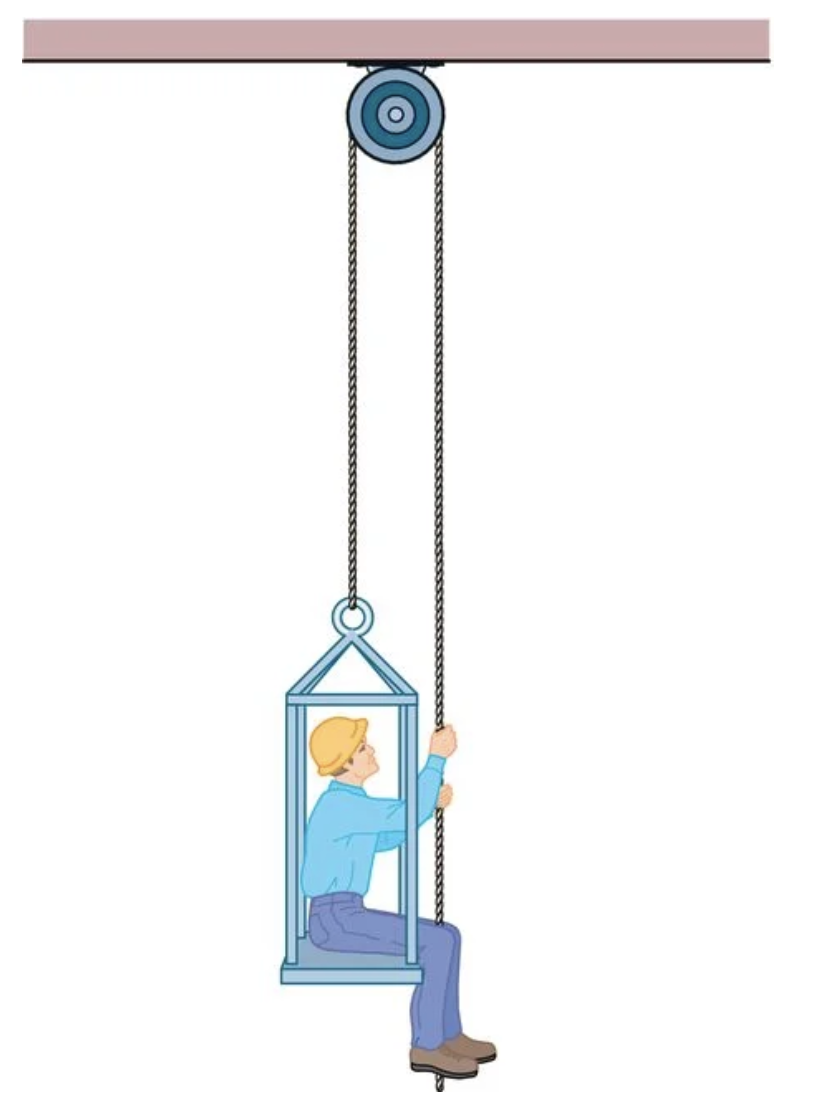
\includegraphics[scale=0.3]{bosun}
\end{frame}

\begin{frame}{Another Menacing Pulley Problem}
\scriptsize


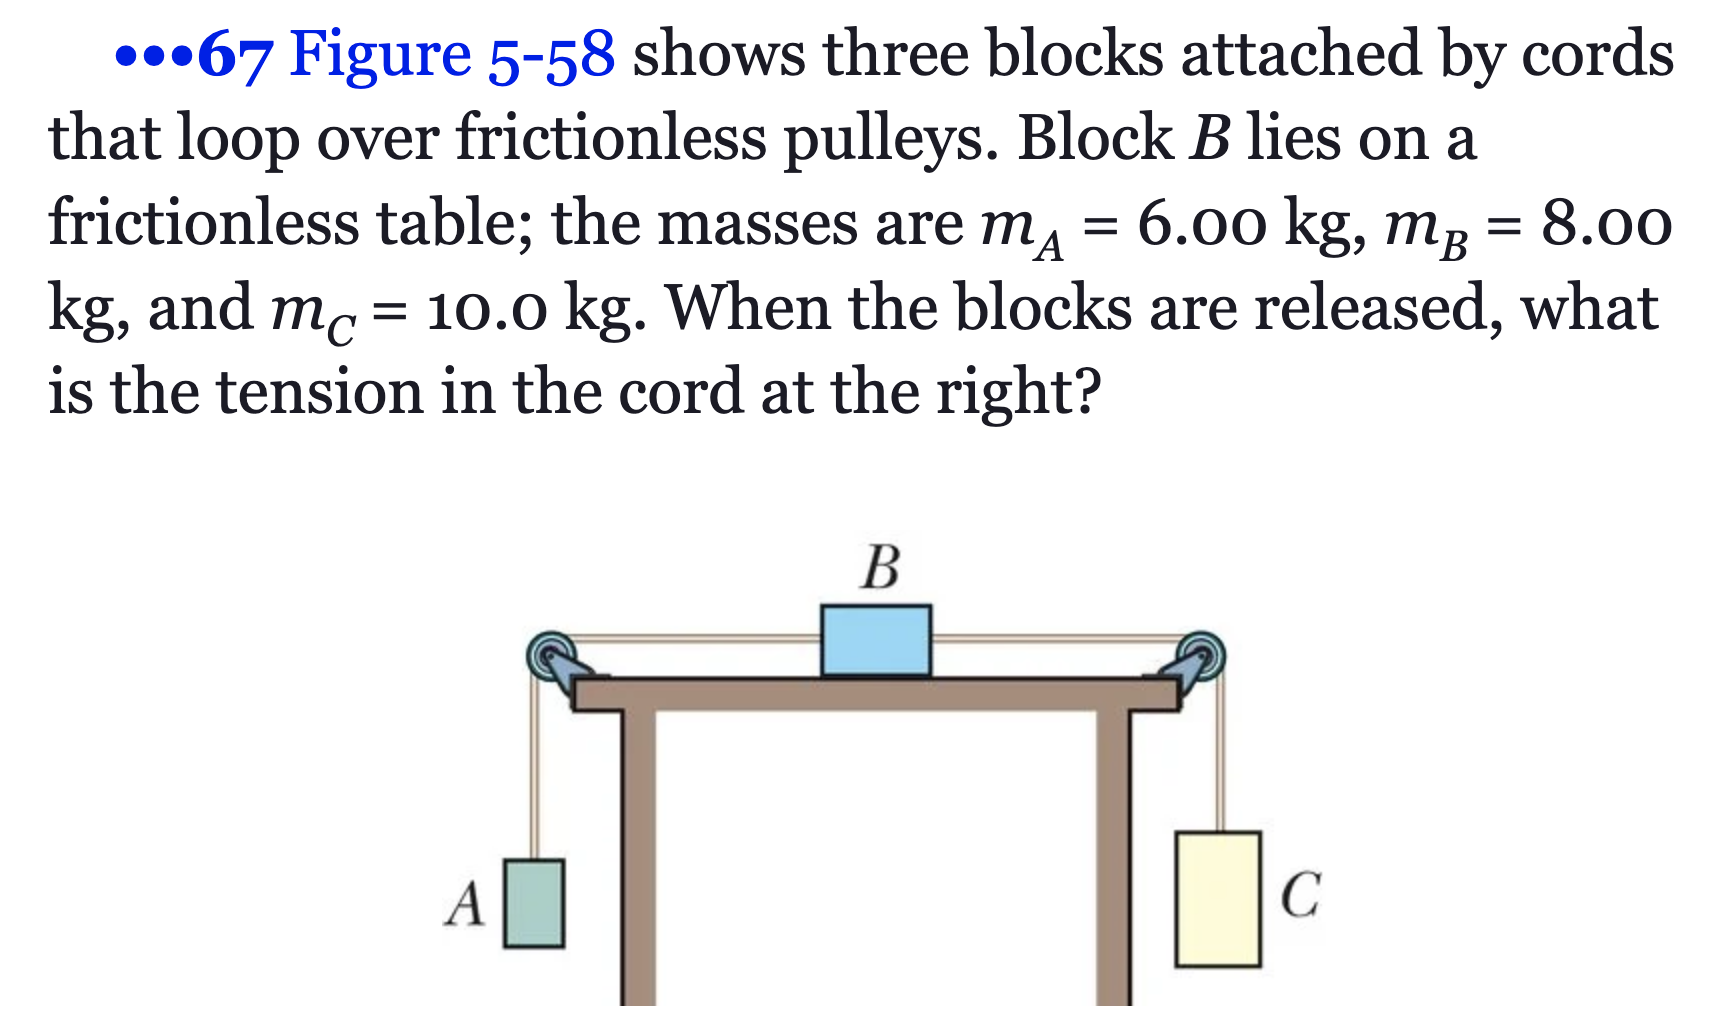
\includegraphics[scale=0.25]{ballots}
\end{frame}
%\begin{frame}{Crate on ramp problems}
%\small
%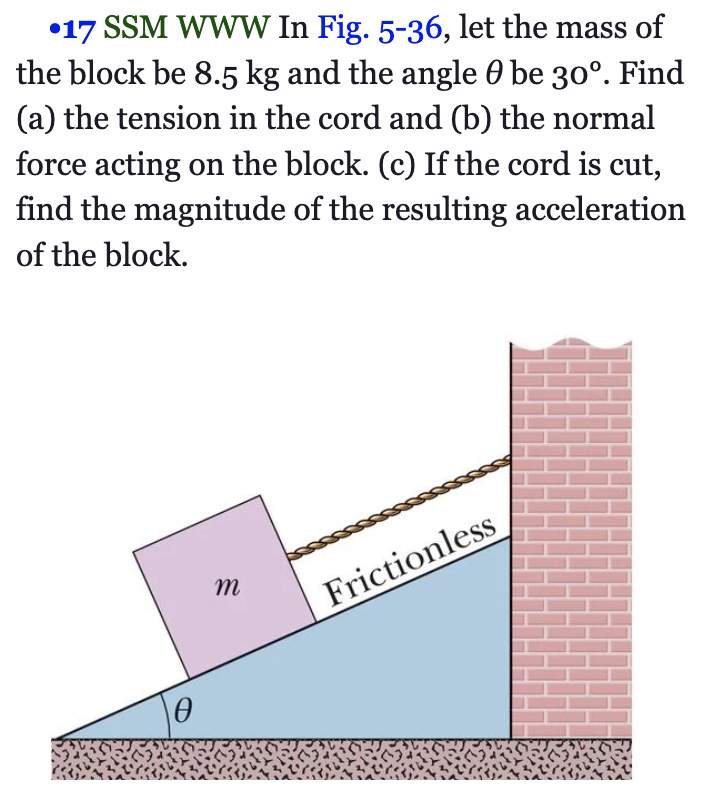
\includegraphics[scale=0.3]{crate1}
%\end{frame}
%

%
%\begin{frame}{Crate on ramp problems}
%\small
%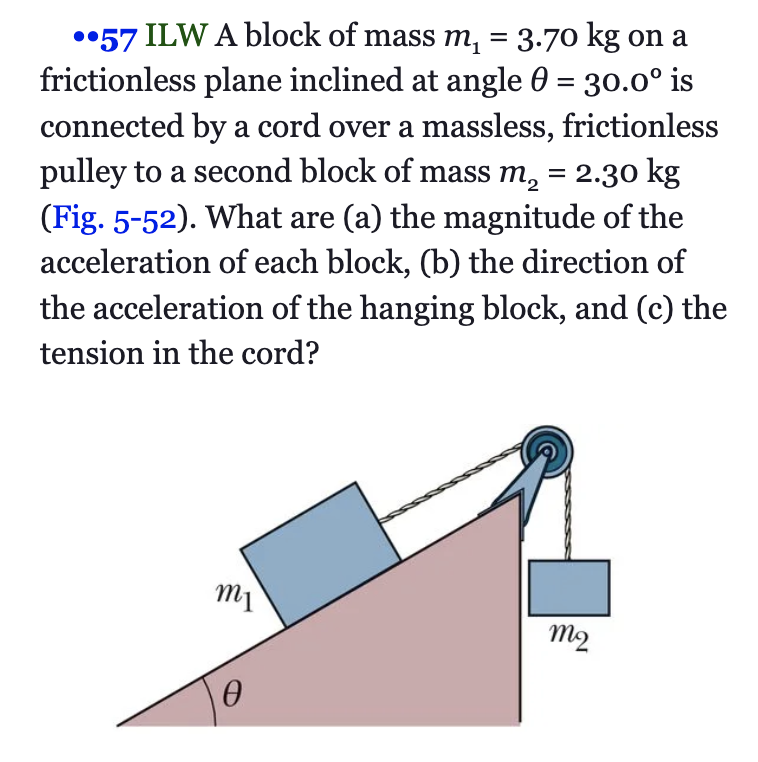
\includegraphics[scale=0.3]{crate3}
%\end{frame}

%\begin{frame}{}
%
%Week 5
%
%\end{frame}
%
%
%
%\section{M\&R 5: Forces 2}
% 
% \subsection{Friction \& Drag}
% 
%\begin{frame}{Friction}
%\small
%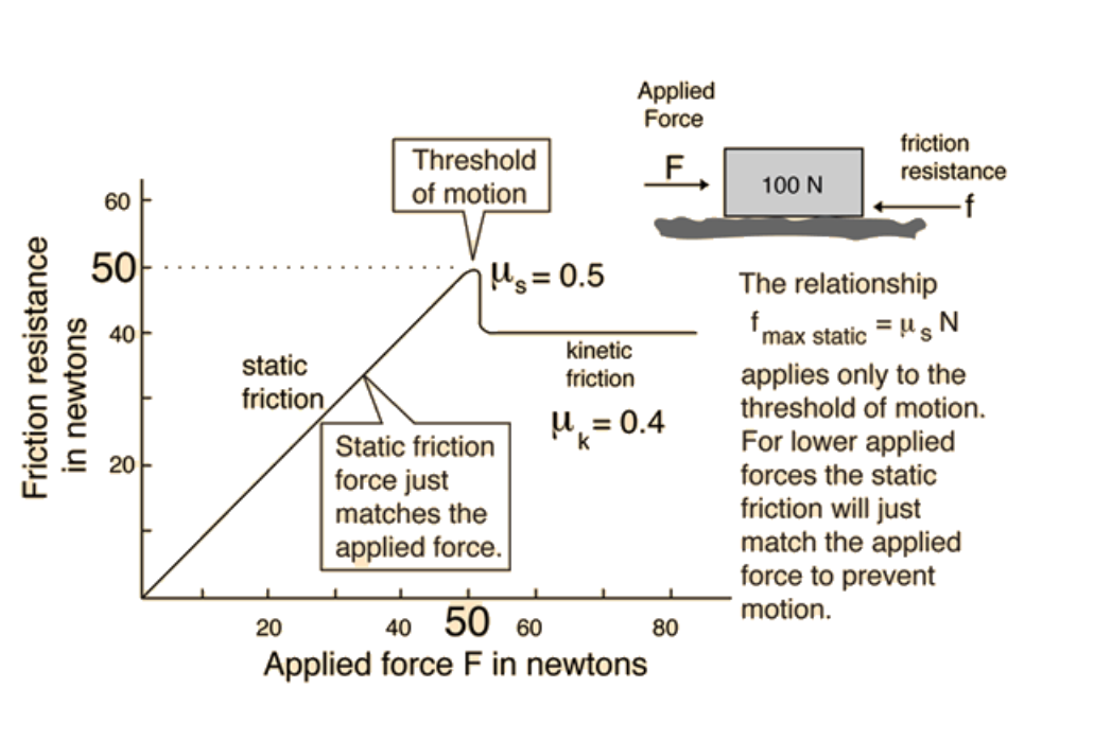
\includegraphics[scale=0.5]{fricpic}
%\vspace{10cm}
%
%\end{frame}
%
%\begin{frame}{Drag}
%\Large
%
%\begin{center}
%
%$F_D = \frac{1}{2} C_D \rho A v^2$
%\end{center}
%\vspace{5cm}
%
%\end{frame}
%
%\begin{frame}{A Problem}
%
%
%\end{frame}
%
%
%
%\begin{frame}{Terminal Velocity}
%\Large
%
%\begin{center}
%
%$v = \sqrt{ \frac{2mg}{C_D \rho A} }$
%
%\end{center}
%
%
%\end{frame}
%
%
%\begin{frame}{A Problem}
%
%
%\end{frame}
%
%
%
%\begin{frame}{Force and UCM}
%\small
%
%\vspace{10cm}
%
%\end{frame}
%
%
% \subsection{Kinetic Energy, Work \& Springs}
%
%\begin{frame}{Work done by a constant Force}
%\small
%$W = \vect{F}\cdot \vect{s} =$ \\[1ex]
%
%\vspace{10cm}
%
%\end{frame}
%
%
%\begin{frame}{Kinetic Energy and Work}
%\small
%
%\vspace{10cm}
%
%\end{frame}
%
%\begin{frame}{Springs}
%\small
%
%\vspace{10cm}
%
%\end{frame}
%
% \subsection{Problems}
%
%\begin{frame}
%Week 5 Thursday Problems:TBD
%\end{frame}


\end{document}